\documentclass[10pt,letterpaper]{article} 
\usepackage{tikz}
\usepackage{tools}
\usepackage{enumitem,caption}
\usepackage{listings}
\lstset{language=Python}
%\lstset{frame=lines}
%\lstset{caption={Insert code directly in your document}}
\lstset{label={lst:code_direct}}
\lstset{basicstyle=\footnotesize}

%\usepackage{graphicx}‎‎
%\usefonttheme{serif}‎
%\usepackage{ptext}‎
%\usepackage{xepersian}
%\settextfont{B Nazanin}
\usepackage{lipsum}
\setlength{\parindent}{0pt}
\newcommand{\pf}{$\blacksquare$}

\newcommand{\Span}{\text{Span}}
\newcommand{\NF}{\text{NF}}
\newcommand{\EDFA}{\text{EDFA}}
\newcommand{\ASE}{\text{ASE}}

\newcommand{\bns}{\textit{broadcast-and-select}  architecture}
\newcommand{\Bns}{\textit{Broadcast-and-select} architecture}

\newcommand{\rns}{\textit{route-and-select} architecture}
\newcommand{\Rns}{\textit{Route-and-select} architecture}

\newcounter{QuestionNumber}
\setcounter{QuestionNumber}{1}

\newcommand{\temp}{{\color{red}{temp}}}

\newcommand{\Q}{
\textbf{Question \theQuestionNumber)}
\stepcounter{QuestionNumber}
}
\newcommand{\EX}{\Bbb E}
\newcommand{\nl}{\newline\newline}
\begin{document}
\large
\begin{center}
In the name of beauty

The 6th problem set of Optical Networks course
\hl
\end{center}
\Q
\begin{enumerate}[label=\alph*-]
\item
Two paths are calculated between a given pair of source and destination. Path 1 has a total length of 2300km and requires 2 regenerations. Path 2 has a total length of 2700km and requires 2 regenerations. Which path do you prefer for establishing the connection? Fully explain about your choice. Is your answer dependent on whether the O-E-O or all-optical architecture does the optical network have? Why or why not?
\item
What is the difference between routing and wavelength assignment (RWA) and routing and spectrum assignment (RSA)? Compare them versus complexity and optimality with enough reasoning.
\item
What type of regeneration (3R or 1R) takes place on signal when passing through a back-to-back transponder structure? What about amplifiers?
\item
It might be thought that the number of regenerations (taken place in nodes) along a path, depends only on optical reach, that said, a path of length 3000km would require one regeneration for an optical reach of 2000km. Bring an example such that a path of length 3000km requires three regenerations, instead of one, for an optical reach of 2000km. What are the possible reasons of extra regenerations?
\end{enumerate}
\Q

In the following network, run
\begin{enumerate}[label=\alph*-]
\item
the Bhandari algorithm
\item
the Suurballe algorithm
\end{enumerate}
 to obtain the shortest path between nodes A and Z (You need not run Dijkstra or Bellman-Ford algorithms separately, only use their results at each step).
\begin{figure}[h]
\centering
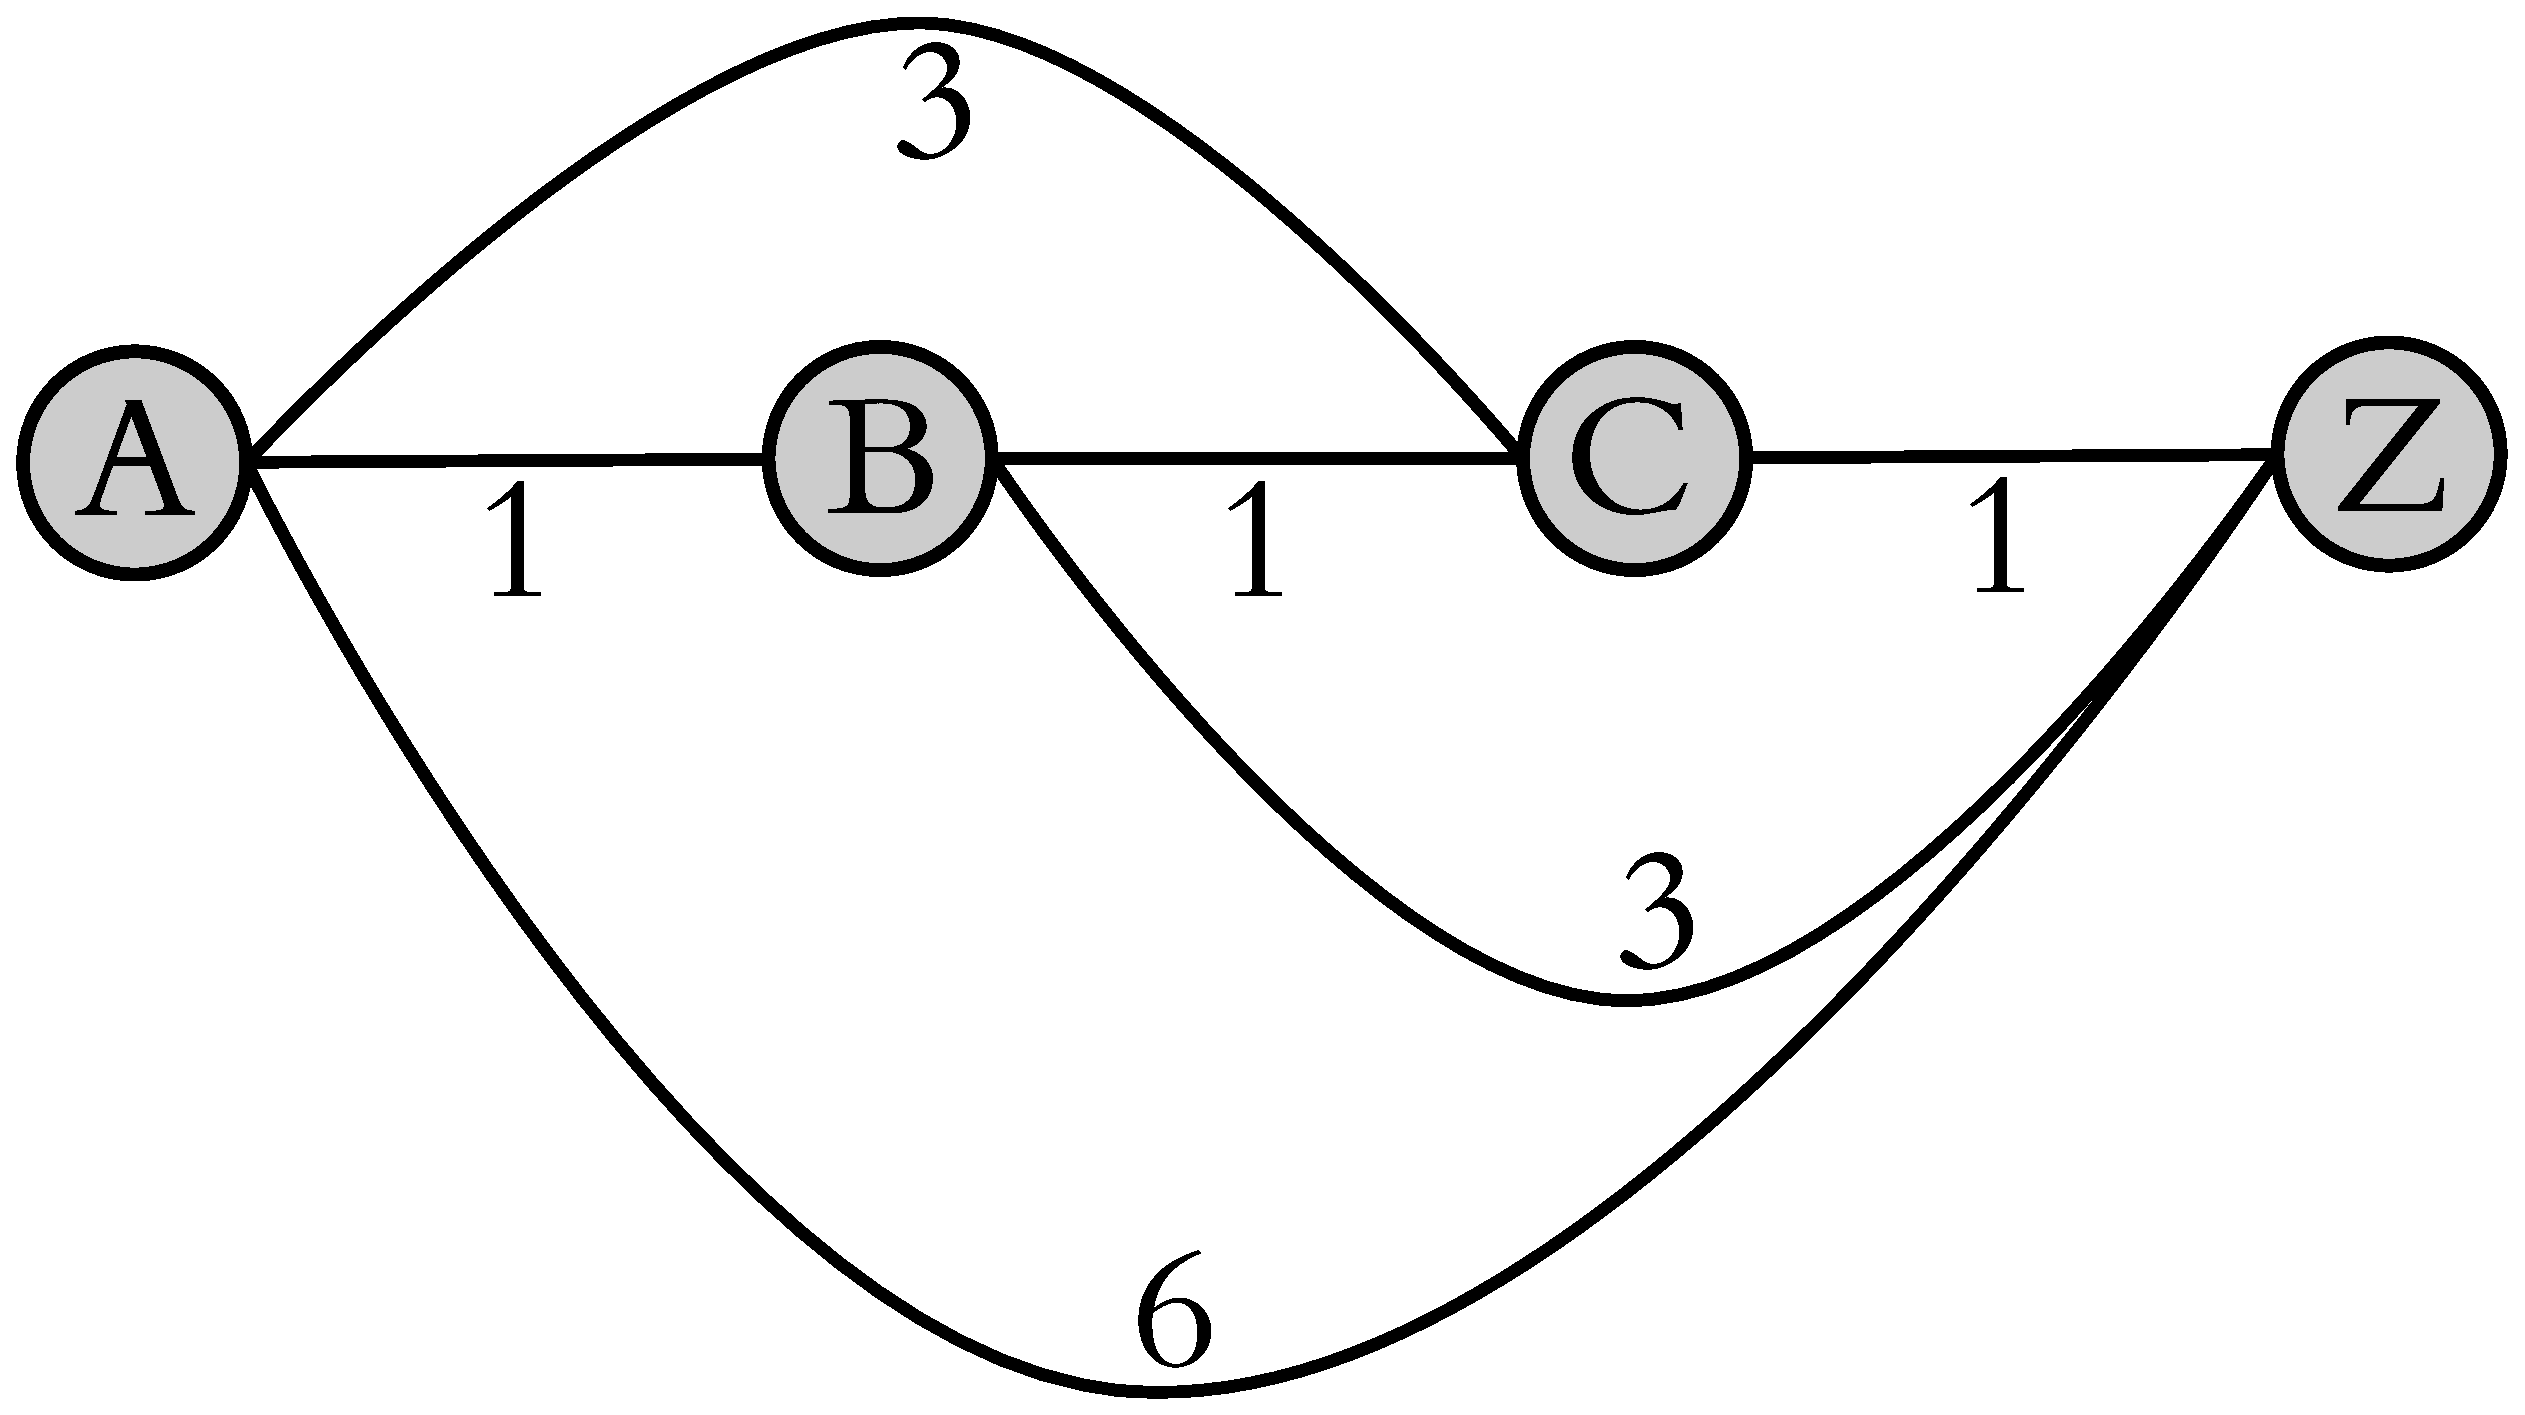
\includegraphics[width=80mm]{bhandari_suurballe1}
\end{figure}

\Q

Assume that a system has a hybrid two-stage amplifier, where the first stage is
Raman based, with a maximum gain of 18 dB, and the second stage is EDFA
based, with a maximum gain of 7 dB. Assume that the amplifier is placed at
the end of a span that has a total loss of 20 dB, and assume that the net gain,
after both stages of amplification, should be 0 dB. The Raman amplification
is distributed over the fiber span that precedes it (i.e., treat the fiber span and
the Raman amplifier as one stage). At 13-dB Raman gain, the NF for the first
stage is 21 dB; assume that the NF decreases linearly by 0.25 dB for every
1-dB increase in Raman gain. The NF of the EDFA stage is fixed at 6 dB regardless
of its gain. What should the gain settings be for the Raman and EDFA
portions of the amplifier to minimize the overall NF, and what is the overall
NF of the two-stage amplifier?

\Q

In the following network, we wish to find the minimum-spanning tree between multicast nodes A, C, E, F and G.
\begin{figure}[h]
\centering
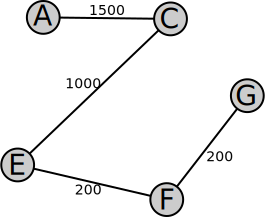
\includegraphics[width=80mm]{steiner}
\end{figure}

Perform the following steps to obtain this tree using MSTE heuristic:
\begin{enumerate}[label=\alph*-]
\item
Create a new physical topology B that contains only the multicast nodes. Any two nodes in B are connected through a link whose metric is equal to the shortest-path distance between those nodes.
\item
Over topology B, find the minimum-spanning tree visually (i.e. no algorithm required).
\item
Expand each link between two nodes of the previous spanning tree into the shortest path in the true topology between those nodes. Call the new topology B'.
\item
Create a new topology (just similar to B) that contains the new nodes (i.e. multicast nodes and nodes on the shortest paths expanded) where link metrics are the shortest path lengths between two nodes. Call this topology C.
\item
Iterate over the same steps of (b) to (d) on topology C as long as no more changes are made, where a minimum-spanning tree has been obtained in the true topology.
\end{enumerate}
(For further reading, refer to the MSTE heuristic method in section 3.10.1 of J. M. Simmons, ``Optical Networks Design and Planning'')
\end{document}